\chapter{Exam II}
\label{ch:exam2-fillin}

\begin{preamble}
\begin{itemize}
\item This exam has 6 question and is worth 100 points.
\item You have 90 minutes to complete the exam after you start.
\item The exam is closed book and you are not allowed to look into your notes and online materials during the exam.
\end{itemize}
\end{preamble}

\section{Miscellaneous}

\begin{problem}[True/False]

Select for each question below whether is it True or False.


%%%%%%%%%%%%%%%%%%%%%%%%%%%%%%%%%%%%
\asktf 

Consider taking the union of two sets with $n$ elements in total
(summed over both sets).  In the worst case, the union operation
performs the most work when the two sets contain an equal number of
elements and less work when one set contains significantly more
elements that the other.

\solt

%%%%%%%%%%%%%%%%%%%%%%%%%%%%%%%%%%%%
\asktf

On an undirected graph if  BFS visits a vertex $v$ at round $r$ (round
start at $0$) then the shortest path from $v$ to the source vertex has
length $r$.

\solt

%%%%%%%%%%%%%%%%%%%%%%%%%%%%%%%%%%%%
\asktf
We can use BFS to find the topological sort of a rooted binary tree.

\solt

%%%%%%%%%%%%%%%%%%%%%%%%%%%%%%%%%%%%
\asktf

When BFS visits a vertex $v$, it adds all of its neighbors to the
frontier, which is to be visited in the next round.

\solf


%%%%%%%%%%%%%%%%%%%%%%%%%%%%%%%%%%%%
\asktf 

In a DFS of a graph, for any edge $(u,v)$ in the graph, the discovery
time of $u$ is less than the discovery time of $v$.  

\solf


%%%%%%%%%%%%%%%%%%%%%%%%%%%%%%%%%%%%
\asktf 
For any DFS-tree edge $(u,v)$ in a graph, the finish time of $v$ is
less than the finish time of $u$.  
\solt

%%%%%%%%%%%%%%%%%%%%%%%%%%%%%%%%%%%%
\asktf 
Given a graph and the DFS numbers, we can determine the
forward, back, and cross edges by inspecting DFS numbers only.  
\solt

%%%%%%%%%%%%%%%%%%%%%%%%%%%%%%%%%%%%
\asktf

If a graph has negative edge weights, the unmodified Dijkstra's
algorithm for shortest path may loop forever.

\solf

%%%%%%%%%%%%%%%%%%%%%%%%%%%%%%%%%%%%
\asktf

If we run Bellman-Ford on a graph with a negative-weight cycle, then
the algorithm will terminate and indicate that it has found a
negative-weight cycle.

\solf
% It can be unreachable from the source.


%%%%%%%%%%%%%%%%%%%%%%%%%%%%%%%%%%%%
\asktf 

A round of graph contraction with star partitioning (star contraction)
eliminates a constant fraction of vertices and edges.

\solf

% not that of edges.

\end{problem}

%% \input{../../../setstables/graph-representation-adj-tables}
\section{(Sets and Tables) Representing Graphs}

\used{S15 exam2, F16}
%uses new set comprehension syntax

\begin{problem}[Adjacency Tables]

Assume for this problem that we represent a directed graph using an
adjacency table representation, where each vertex is mapped to its set
of neighbors. 

Recall that you can use set comprehension syntax for sets and tables.

\ask[5]
Write out the how the graph would be represented in this
representation using the notation for sets and tables that you have
learned in class.

\begin{center}
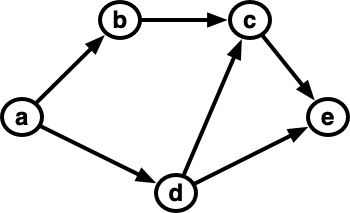
\includegraphics[width=2in]{media/digraph-1.jpg}
\end{center}

\sol
$\{a \mapsto \{b,d\}, b \mapsto \{c\}, c \mapsto \{e\}, d \mapsto \{c,e\}, e \mapsto \{\} \}$ \\

\notes
\textbf{Common Mistakes}: Forgetting to include $e \mapsto \{\}$. 


\ask[12]
Your goal now is to write a function that given a graph creates
another graph where each pair of edges is shortcut.  That is any edge
in the input graph is also in the output graph, and in addition for
any pair of edges of the form $(u,v),(v,w)$ in the input graph $G$,
there is an additional edge $(u,w)$ in the output.

In the code below, you only need to fill in the underlined line. 


%% \begin{lstlisting}[numbers=none]
%% fun shortcut(G) = 
%%   let 


%%     fun f (N,G) = ________________________________________________


%%   in   

%%     {u <- f(N,G): (u <- N) in G }

%%   end

%%\end{lstlisting}

\solfin
\begin{lstlisting}[numbers=none]
fun shortcut(G) = 
  let 
    fun f (N,G) = ____ N union (big_union_(v in N) G[v]) ____
  in   
    {u <- f(N,G): (u <- N) in G }
  end
\end{lstlisting}


\notes

\textbf{Common Mistakes}: Forgetting to include N, the argument passed in into the solution. When writing set notation mixed with SML, forgetting that Table.find returns an option rather than the actual argument. Also, often students forgot to convert between a sequence and a set, which led to using functions such as map on sets.

\end{problem}


\begin{problem}[8.] 

You are given a hash table $T$ with 13 buckets numbered from $0$ to $12$.

\ask Show the contents of $T$ after inserting the keys
$\cseq{16,6,18,5,9,8,5,7,2}$ using open addressing with linear
probing.  The hash function is $h(i) = i \mod 13$.


\solfin

0: \fin{~~~~~~~~}\\
1: \fin{~~~~~~~~}\\
2: \fin{~~~~~~~~2}\\
3: \fin{~~~~~~~~16}\\
4: \fin{~~~~~~~~}\\
5: \fin{~~~~~~~~18}\\
6: \fin{~~~~~~~~6}\\
7: \fin{~~~~~~~~5}\\
8: \fin{~~~~~~~~8}\\
9: \fin{~~~~~~~~9}\\
10: \fin{~~~~~~~~7}\\
11: \fin{~~~~~~~~}\\
12: \fin{~~~~~~~~}\\
\end{problem}

\begin{problem}[8.] 

You are given a hash table $T$ with 13 buckets numbered from $0$ to $12$.

Show the contents of $T$ after inserting the keys
$\cseq{16,6,18,5,9,8,5,7,2}$ using open addressing with linear
probing.  The hash function is $h(i) = i \mod 13$.




\ask 0: \sol ~~~
\ask 1: \sol ~~~
\ask 2: \sol ~~2
\ask 3: \sol ~16
\ask 4: \sol
\ask 5: \sol ~18
\ask 6: \sol ~~6
\ask 7: \sol ~~5
\ask 8: \sol ~~8
\ask 9: \sol ~~9
\ask 10: \sol ~~7
\ask 11: \sol ~~~
\ask 12: \sol ~~~
\end{problem}

\begin{problem}[8.] 
Given the performance given in class for melding two leftift heaps
\texttt{PQ.meld}, give the work and span of the following algorithms for
building a heap from a sequence $S$ of $n$ keys:


\ask
 
\begin{lstlisting}[numbers=none]
  Seq.reduce PQ.meld PQ.empty (Seq.map PQ.singleton S)
\end{lstlisting}

\solfin

$W(n) =  \fin{????????????}$

$S(n) =  \fin{????????????}$

\ask

\begin{lstlisting}[numbers=none]
  Seq.iterate PQ.meld PQ.empty (Seq.map PQ.singleton S)
\end{lstlisting}

\solfin

$W(n) =  \fin{????????????}$

$S(n) =  \fin{????????????}$


\end{problem}


%% \newpage
%% \input{../../../dfs/dfs-numbers-1}
\section{(DFS) Numbers}

Given a graph $G = (V,E)$, the traversal order of a depth-first search starting
from $s$ defines a tree $T(G, s)$, known as the \emph{depth-first search tree},
with the following properties:
\begin{enumerate}[itemsep=2pt,topsep=0pt,label=(\roman*),
  labelindent=2\parindent,
  leftmargin=*]
\item $s$ is the root of the tree $T(G,s)$;
\item the tree $T(G,s)$ contains exactly the vertices reachable from $s$; and
\item there is an arc (a directed edge) from $u$ to $v$ if the
  \emph{first} visit to $v$ is
from $u$ (i.e., $u$ calls DFS on $v$ and $v$ hasn't been visited before).
\end{enumerate}

It is easy to record the \emph{discovery time} $d_u$ and
\emph{finishing time} $f_u$ for every vertex.  Starting with a count
of 1, each time a vertex is
first visited (enter) and when a vertex is
last visited (exit) the counter is incremented.  The discovery time
corresponds to the counter when it is first entered, and the finishing
time corresponds to the counter when it last visited.



Run depth-first search on the directed graph below, starting at vertex
A. Whenever there is a choice in the order to explore vertices, use
the vertices in alphabetical order.
For each vertex fill in the corresponding row in the
table with the discovery and finishing
times for that vertex. For example, at the root node $A$, the
counter is $1$ when it is first visited and $12$ when it is finally exited.



\vspace{.1in}
\noindent
\begin{minipage}{.45\textwidth}
\begin{center}
  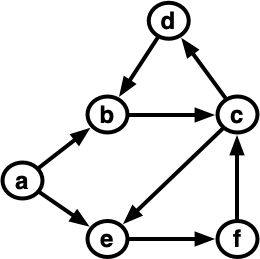
\includegraphics[scale=.45]{media/dfs-numbers.jpg}\\[.2in]
\end{center}
\end{minipage}

\begin{problem}
For each vertex, write its discovery, and finish time

\ask vertex A \solfin discovery: \fin{1} and  finish: \fin{2}. 
\\
\ask vertex B \solfin discovery: \fin{2}  and  finish: \fin{7}.
\\
\ask vertex C \solfin discovery: \fin{3} and finish: \fin{6}.
\\
\ask vertex D \solfin discovery: \fin{4} and finish:  \fin{5}.
\\
\ask vertex E \solfin discovery: \fin{18} and finish: \fin{11}.
\\
\ask vertex F \solfin discovery:  \fin{9} and finish: \fin{10}.
\end{problem}


\begin{problem}[9.]

For each edge, write down whether it is a tree edge or is a
forward', back, or cross

\ask
(A, B)
\solfin \fin{tree}

\ask
(A, B) 
\solfin \fin{tree}

\ask (B, C)
\solfin \fin{tree}

\ask (C, D)
\solfin \fin{tree}

\ask (D, B)
\solfin \fin{tree}

\ask (A, E) 
\solfin \fin{tree}

\ask (E, C) 
\solfin \fin{cross}

\ask (E, F)
\solfin \fin{tree}

\ask (F, C) 
\solfin \fin{cross}
\end{problem}


\begin{problem}[4]

\asktf Is it possible to find a topological order of the vertices
for the above graph?

\solf


\ask 
Justify your answer.
\sol
The graph must be a directed acyclic graph in order to
topological sort the vertices.

\end{problem}


%% \input{../../../shortest-paths/shortest-paths-basics}

\section{Shortest Paths, The Basics}
\used{S15 exam2}

This problem concerns several basic properties of shortest paths and
shortest path algorithms that we saw in class, Dijkstra's and
Bellman-Ford.

\begin{assumption}
Assume that the graphs contain no negative edges and are
represented using adjacency sequences,  which map each
vertex to the sequence of out-neighbors and edge weights.

Use $n$ for the number of vertices in the graph and $m$ for the number
of edges.
\end{assumption}



\begin{problem}[Work and Span]

Let $G$ be a graph and a source vertex $s$ such that all vertices in
the graph are connected via a shortest path to $s$ that contains $k$
or fewer edges.

\ask
What is the work and span of an execution of Dijkstra's algorithm on
$G$ and $s$?

\solfin 
Work: \fin{$O(m\log{n})$}
Span: \fin{$O(m\log{n})$}

\ask
What is the work and span of an execution of Bellman-Ford algorithm on
$G$ and $s$?

\solfin
Work: \fin{$O(km)$}
Span :  \fin{$O(k\log{n})$}

\notes
\textbf{Common Mistakes:}
\begin{itemize}
	\item Not recognizing that there are only $k$ rounds of Bellman Ford in this
  scenario.

	\item Including an extra factor of $O(\log n)$ in the work. (This is
  eliminated when the graph is represented by an adjacency sequence.)
\end{itemize}
\end{problem}

\begin{problem}
Recall that a {\em single-pair} shortest path query asks for the
shortest path from a source to a destination.
%

In many applications of shortest paths, we repeat single-pair queries
on the same graph $G = (V,E)$ and often with a small number $k$ of
{\em special} sources, where $k \ll n$ ($k$ is very small relative to
$n$).


One way to take advantage of this use case is to pre-process the graph
in some way to generate some data structure (possibly another graph)
based on the $k$ special sources, and then use this data structure to
answer the shortest path queries.


\ask[4] Describe a preprocessing algorithm that takes a graph
  and the special sources as input and computes the data structure (2-3
  sentences should suffice).  Your preprocessing algorithm should be
  parallel and should perform as little work as possible.


\sol

  Assuming that \textsf{Dijkstra$(G, s)$} returns a mapping of vertices to
  their shortest-path distances (or shortest paths themselves), starting from
  source $s$:
  \[
    \big\langle (\textsf{if $v$ is a special source then Dijkstra$(G,v)$
    else $\bot$}) : v \in V \big\rangle
  \]

 For each source vertex in the source set, perform Dijkstra, all in
 parallel.  Create a graph that contains all the vertices of the
 original graph and a $k(n-1)$ edges from each source to all other
 vertices, where each edge has a weight that is equal to the shortest
 path that it represents.


\rubric Using Bellman-Ford is overkill. No more than 1 points for
that. Instead of the graph, we can also create a table mapping sources
do distances (this is the same things as the graph). For efficiency
though the table should be represented as a sequence of sequences.  If
this is not mentioned, then take out $-1$.

\notes
\textbf{Common Mistakes:}
\begin{itemize}
  \item Not specifying which shortest path algorithm to use.
  \item Using Bellman-Ford rather than Dijkstra. We are guaranteed non-negative
  edge weights, so Bellman-Ford is too expensive.
  \item Ambiguity in describing what happens in parallel.
  \item Unable to guarantee fast query (see below).
\end{itemize}


\ask[4]
State the work and span of your algorithm

\solfin 
Work: \fin{$O(n + km\log n)$}
Span: \fin{$O(m\ log n)$}

\ask[5]
Describe how to use the data structure resulting from the
preprocessing algorithm to answer quickly and efficiently single-pair
shortest path queries originating at one of the special sources (no
restrictions on the destination)

\sol
If $D$ is the result of the preprocessing step and we are looking for a path
$(s, t)$, then simply perform a lookup: $D[s][t]$.
~~~~~~~~~~~~~~~~~~~~~~~~~~~~~~~~~~~~~~~~~~~~~~~~~

\notes
\textbf{Common Mistakes:}
\begin{itemize}
	\item Query is too expensive, due to insufficient preprocessing.
	\item Query is unable to distinguish between different source vertices, due
  to simplifications made in the preprocessing step. For example, if all
  sources were combined into a single node, or if they were all connected to
  some new unique source via weight-0 edges.
	\item Attempting to reconstruct paths, resulting in a cost of $O(d)$, where
  $d$ is the diameter of the graph. We should instead just construct paths in
  the preprocessing step.
	\item Incurring a logarithmic lookup cost, due to using tables. Sequences are
  sufficient, and we get constant-time lookup.
\end{itemize}


\ask What is the work and span of your algorithm Work: 
\solfin 
Work:  \fin{$O(1)$} 
Span: \fin{$O(1)$} 


\end{problem}




%% \newpage
%% \input{../../../shortest-paths/bounded-hops}

\section{(Shortest Paths) Bounded Hops}

In many real-world road networks, the shortest paths between points of
interest include a small number of edges.  This is because if there
are too many edges on a route, we build a highway that enables
shortcutting past them.  

Suppose you are given a weighted graph $G$ in which the shortest path
between any two vertices has $t$ or fewer edges and answer the
following questions.  The graph can contain negative edges.

For cost bounds you can assume that the vertices are labeled as $0
\ldots n-1$, where $n$ is the number of vertices; $m$ denotes the
number of edges.

\begin{problem}[6.]

\ask
Describe an algorithm for solving the single-source shortest %
path problem for such a graph.  Your algorithm should be efficient
with a work bound that depends on $t$ (and other graph parameters).

\sol
You can use Bellman-Ford algorithm as given in class, which stops
after $t$ iterations by detecting no changes in distances, or use a
version that stops after $t$ iterations without further checking.

\ask
Argue that your algorithm is correct.

\sol
  The algoritm is correct because at iteration $i$, we know that
  Bellman-Ford finds all shortest path with $i$ or less hops.  It will
  therefore stop after $t$ iterations.
\end{problem}


\begin{problem}[2.]

Describe the cost specifications that you would use (e.g., array sequences, treap tables, etc) to implement your algorithm,
and its work and  span.

\ask Cost specifications
\sol Array sequences~~~~~~~~~~~

\ask Work 
\sol  work is $O(tm)$ and 
\ask Span 
\sol  span is $O(t\log{n})$.
\end{problem}


\begin{problem}[4.]

You are now concerned only with graphs with positive edge
weights. 

\ask[2.]
Describe an algorithm that solves the single-source shortest
paths problem by performing no more than $\min ( \log{n}, \, {t} )
\cdot {m}$ work.  \vspace{1in}

\sol
  If $t$ is less that $lg n$ then run (the modified) Bellman-Ford
  algorithm.  If not, then just use Dijkstra's algorithm.


\ask[2.]
Argue why your algorithm satisfies the given work bound.

\sol
  The algorithm satisfies the work bound trivially because it reverts
  to Dijkstra for cases when the hop count exceed $\log n$.

\end{problem}


%% \input{../../../graph-contraction/edge-contraction-on-binary-trees.tex}

\section{Tree Contraction via Edge Contraction}

In class you have seen that graph contraction with edge partitions is
not efficient because it can fail to eliminate a constant fraction of
the vertices in a round.  
%
In this question, you will explore whether edge contraction would work
for (rooted) binary trees.

Let's start with a basic definition. 
%
In a (rooted) binary tree, each node has zero, one or two children. 
%
We say that
a node is {\em binary} if it has two children, {\em unary} if it has
one child, and {\em leaf} if it has no children.  
%


Throughout use the following notation for a given binary tree:
%
{
\flushleft
\begin{minipage}[b]{4in}
\begin{itemize}
\item $n$ is the number of nodes in the tree,
\item $\ell$ is the number of leaves in the tree, 
\item $n_u$ is the number of unary nodes in the tree, and 
\item $n_b$ is the number of binary nodes in the tree.
\end{itemize}
\end{minipage}
\begin{minipage}{2in}
\begin{center}
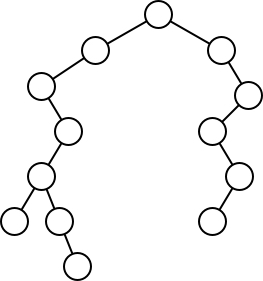
\includegraphics[width=1.7in]{media/binary-tree.jpg}
\end{center}
\end{minipage}
}


\subsection{Leaves and Binary Nodes}

\begin{problem}
The number of leaves in a binary tree  is equal to some function $\mathit{leaves}(n_b)$
of the number of binary nodes in this tree.
%

\ask[4]
State this function.
%
\[
\mathit{leaves}(n_b) = 
\]

\sol
\[
\mathit{leaves}(n_b) = \underline{n_b + 1}
\]
\end{problem}

\begin{problem}
Prove the property by structural induction.

\ask IH: 
\sol 
We shall prove by induction that in a binary tree the number of
leaves is at most $n_b + 1$, where $n_b$ is the number of binary nodes.

\ask Base case (a leaf)

\sol
In the base case we have a single leaf and $n_b = 0$.

\ask Inductive case:

\sol

Now consider a binary tree with greater than one node. 

\begin{itemize}
\item Case I:  The root is a binary node. Let $l_1$ and $l_2$ the number of leaves
and let $b_1$ and $b_2$ be the number of binary nodes in the two
subtrees.  We know, by induction, that $l_1 = b_1 + 1$ and $l_2 = b_2
+ 1$ and thus we have $l_1 + l_2 = b_1 + b_2 + 2$, which is one more
than the number of binary nodes in the tree ($b_1 + b_2 + 1$).

\item Case II: The root is a unary node.  Let $l$ be the number of
leaves in the subtree rooted at the child of the root. By induction we
know that $l = b + 1$, where $b$ is the number of binary nodes in the
tree. The lemma holds trivially for the tree, because $l$ and $b$ are
the same.
\end{itemize}
\end{problem}


\subsection{Edge Contraction}
You will now apply the randomized edge contraction to binary trees.

\begin{problem}
\ask[2.]
Describe the randomized edge partition technique that you have seen in
the lecture (also available in your notes). 

\sol
Flip a coin for each edge. If it comes up heads and all the edges
incident on the two endpoints come up tails, then select the edge.


\ask[5.]
Out of the edges incident on leaves, give a lower bound on the
fraction that will be selected, in expectation.

\sol
Let $v$ be a leaf and $u$ be its parent. If $u$ is unary, then the
edge will be selected with probability at least $1/4$.  If $u$ is
binary, then it will be selected with probability at least $1/8$.
Therefore at least $1/8$ of all the edges will be selected.




\ask[5.]
Out of the edges from a unary node to its parent, give a lower bound
on the fraction that will be selected, in expectation.

\sol
\begin{itemize}
\item Case I: If the parent is unary, then the probability is $1/8$.
The edges that must agree are to the child, to the parent, to the
grandparent from the parent.
\item Case II: If the parent is binary, then the probability is
$1/16$. The edges that must agree are like above but we have one more
edge between the parent and our sibling.
\end{itemize}

Note that if the parent doesn't have 

Thus the lower bound is $1/16$.


\end{problem}

\begin{problem}[4.][Extra credit]
\ask
Can you combine the your solutions to the two parts above to argue
that a binary tree can be contracted efficiently and in parallel.

\sol
Yes, we will ignore edges from a binary node to its parent but we will
apple edge contraction to the edges that are between leaves and unary
nodes and their parents.  The key observation is that if we apply edge
contraction to these than we can recur, because the resulting
tree remains to be binary.

As shown above each of these are deleted by a constant fraction.  The
question is can the unary and the leaves constitute a constant
fraction of all the edges.  The answer is yes, because we know that we
have at most $\ell$ binary nodes.  
\end{problem}
